\chapter{Move Generation}
\label{move generation} %\label{1cap:spinta_laterale}
% [titolo ridotto se non ci dovesse stare] {titolo completo}
%

\begin{citazione}
    In questo capitolo viene mostrato passo passo un procedimento guida alla realizzazione di un motore scacchistico
\end{citazione}
\newpage


\section{Introduzione} %\label{1sec:scopo}
Una volta stabilito il tipo di rappresentazione il passo successivo è quello della generazione delle mosse,per generazione delle mosse si intende la generazione
di tutte le mosse legali eseguibili data una posizione di partenza , la generazione delle mosse è un processo fondamentale in quanto identifica i rami che
il nostro algoritmo potrà esplorare nella successiva fase, quella appunto di ricerca, trattata nel capitolo \ref{ricerca}.



\section{Struttura di una mossa}%\label{1sec:scopo}
Prima di parlare della generazione delle mosse, iniziamo col parlar e della struttura di una singola mossa,un requisito fondamentale che ogni rappresentazione di una mossa deve avere,
è la scelta di una rappresentazione conforme con quella scelta per la codifica della scacchiera e dei pezzi,trattandosi di un elemento realizzabile in moltissimi modi, con tante soluzioni di simile efficienza,
non verrà fornito un elenco esaustivo delle possibili scelte ma verrà trattata solo una rappresentazione d'esempio.


\begin{figure}[h]
    \centering
    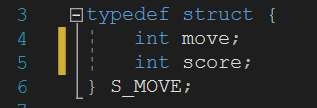
\includegraphics[width=\linewidth/2] {move.png}
    \caption{move.h}
\end{figure}

Ogni mossa è memorizzata come un intero di 32 bit ( con 25 bit effettivamente utilizzati):
\begin{itemize}[leftmargin=*]
    \item  0000 0000 0000 0000 0000 0\textbf{111 1111} -> La casella di partenza è codificata con 7 bit,assume il valore 0-127 dell'indice da cui il pezzo viene mosso
    \item 0000 0000 0000 00\textbf{11 1111 1}000 0000 ->  La casella di arrivo  è codificata con 7 bit,assume il valore 0-127 dell'indice in cui il pezzo viene mosso
    \item  0000 0000 00\textbf{11 11}00 0000 0000 0000 -> In caso di cattura, il tipo di pezzo catturato viene codificato in 4 bit,assume il valore 0-15 del tipo di pezzo catturato (0 codifica una mossa senza cattura)
    \item 0000 0000 0\textbf{1}00 0000 0000 0000 0000 -> Un bit è utilizzato per codificare se  la mossa è una presa en passant
    \item 0000 0000 \textbf{1}000 0000 0000 0000 0000 -> Pawn Start 0x80000,   1 to  store if it was a pawn start
    \item 0000 \textbf{1111} 0000 0000 0000 0000 0000 -> In caso di promozione di un pedone,il tipo di pezzo nel quale il pedone è stato promosso è codificato in 4 bit
    \item 000\textbf{1} 0000 0000 0000 0000 0000 0000 -> Un bit è utilizzato per codificare se  la mossa è un arrocco
\end{itemize}
Inoltre insieme alla rappresentazione della mossa viene anche conservato un valore intero nel quale conservare la "bontà" della mossa,ossia quanto riteniamo che la mossa
sia promettente nel futuro della ricerca e che verrà calcolato nella fase di valutazione, trattata nel capitolo \ref{valutazione}.

\subsubsection{Lista delle mosse}
Una volta definita la struttura di una singola mossa, definiamo anche una struttura chiamata movelist che consiste nella lista di tutte le mosse registrate dall'inzio della partita e da un contatore delle stesse,infine definiamo delle bitmask utili ad estrarre specifiche informazioni da una mossa
\begin{figure}[h]
    \centering
    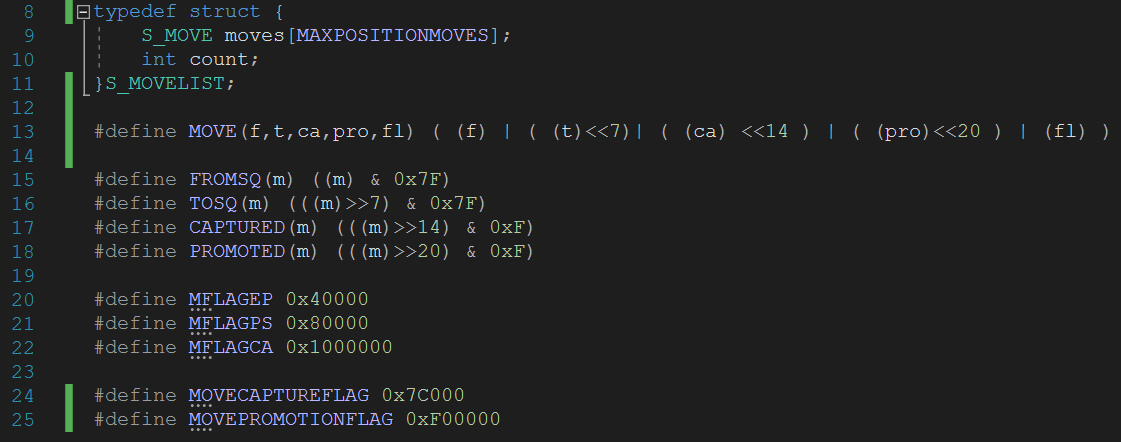
\includegraphics[width=\linewidth/2] {movelist.png}
    \caption{struttura movelist e bitmasks presenti in move.h }
\end{figure}





\LARGE{movegen.c usa attack.c, Va spiegato.}
\normalsize





\section{Generare le mosse}

In questa sezione verrà trattata la generazione delle mosse,prima di iniziare a parlare della generazione però è debito soffermarsi su come le mosse ,una volta generate, vengono aggiunte alla lista di possibili mosse.
Definiamo in movegen.h una funzione per l'inserimento  per ogni tipo di mossa possibile che potrà essere creata durate la generazione delle stesse:

\begin{figure}[H]
    \centering
    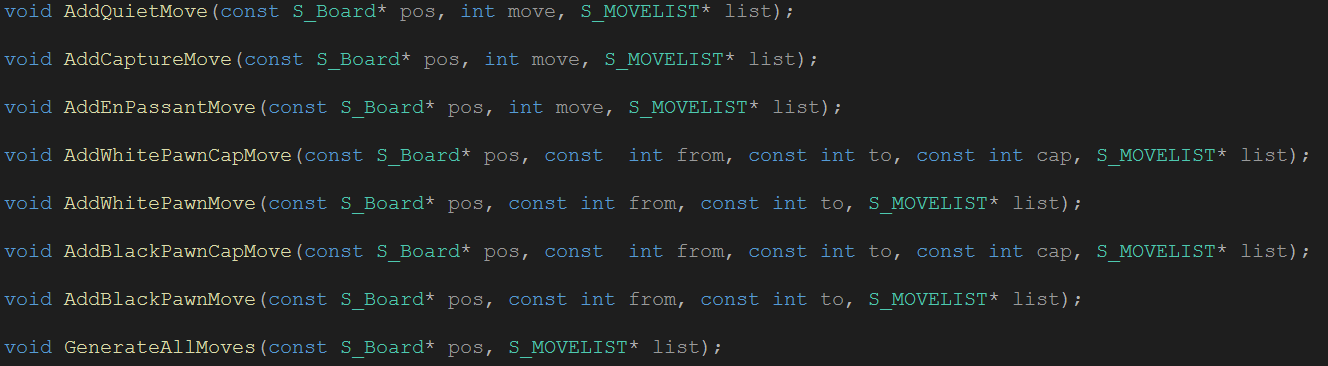
\includegraphics [width=\linewidth]{movegen-h.png}
    \caption{movegen.h }
\end{figure}

Come si può notare dai nomi delle funzioni,negli scacchi le mosse sono divise in due categorie,
le mosse possono essere "quiet/silenziose" o meno , sono "silenziose" tutte le mosse che non risultano in una cattura o in una promozione.
Abbiamo quindi due funzioni, una chiamata "AddQuietMove" che si occupa dell'aggiunta delle mosse silenziose ed una chiamata "AddCaptureMove" che gestisce le altre.  

\begin{figure}[H]
    \centering
    \includegraphics [width=\linewidth]{immagine.png}
    \caption{movegen.h }
\end{figure}

Discorso a parte va fatto per i pedoni,i pedoni sono il pezzo più difficile da trattare in quanto, come vederemo anche nel paragrafo \ref{pedoni}
è l'unico pezzo che può catturare con en passant e che può promuovere,creiamo quindi delle funzioni che gestiscono la possibilità del pedone di poter essere promosso in uno qualsiasi dei 4 pezzi
aggiungendo di fatto 4 mosse invece di 1,di seguito sono riportate le funzioni per il pedone bianco, quelle del pedone nero sono identiche con ovviamente gli enum cambiati per rispecchiare la differenza.
\begin{figure}[H]
    \centering
    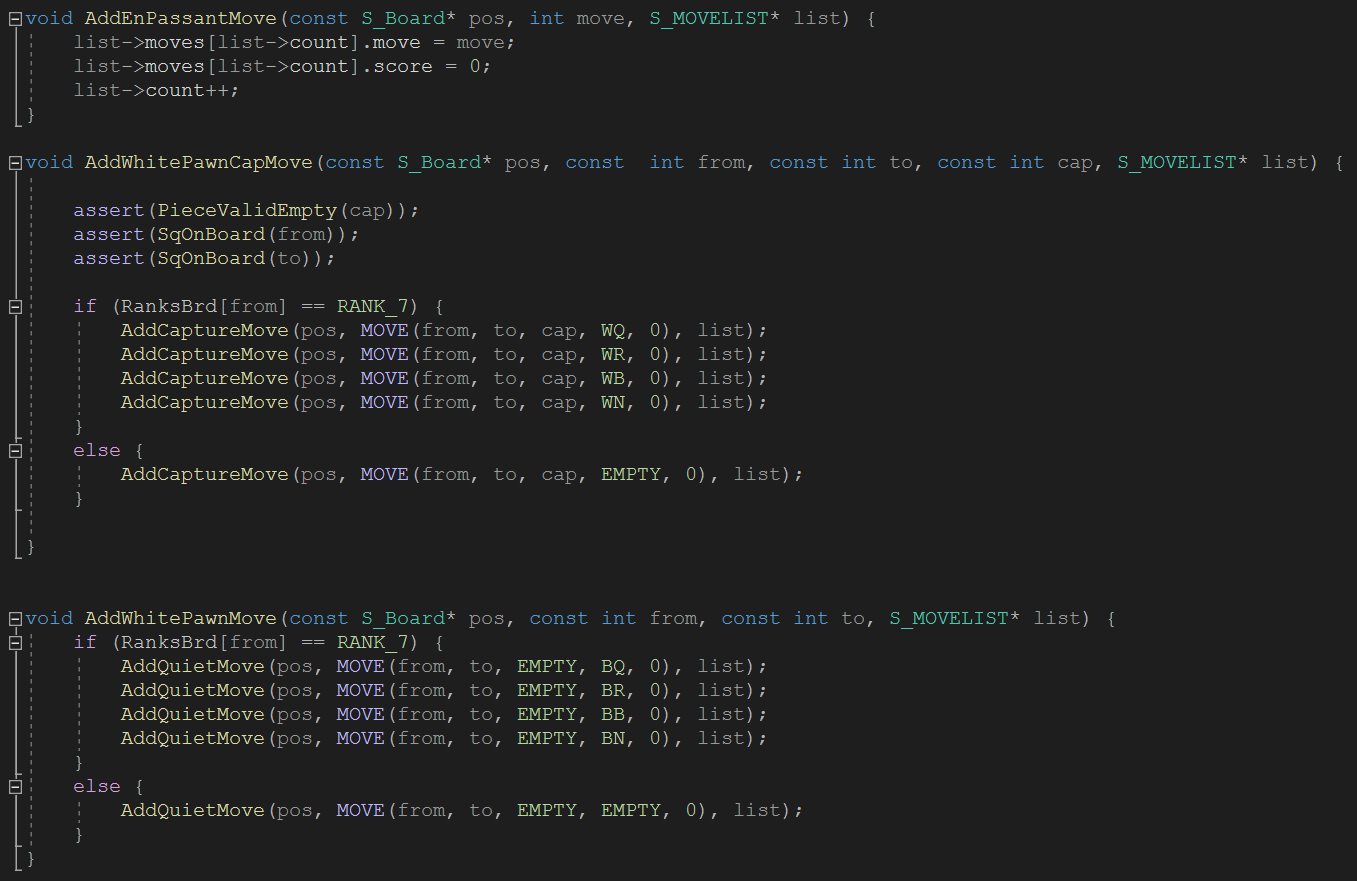
\includegraphics [width=\linewidth] {PawnMoves.png}
    \caption{move.h}
\end{figure}



\subsection{Pedoni}\label{pedoni}
Il pedone muove solo in avanti, mai indietro o di lato. Un pedone può avanzare  di due caselle se è la prima volta che viene mosso,altrimenti può avanzare solo di una casella.
Il un pedone mangia un pezzo avversario spostandosi diagonalmente di una casella,sempre soltanto in avanti, o a destra o a sinistra, se un pedone raggiunge la traversa finale della scacchiera rispetto alla sua direzione di movimento
allora viene promosso, diventa quindi,a scelta del giocatore che possiede la pedina, uno qualsiasi degli altri pezzi  (ad eccezione del re).

\begin{figure}[H]
    \centering
    \begin{minipage}[b]{0.21\textwidth}
        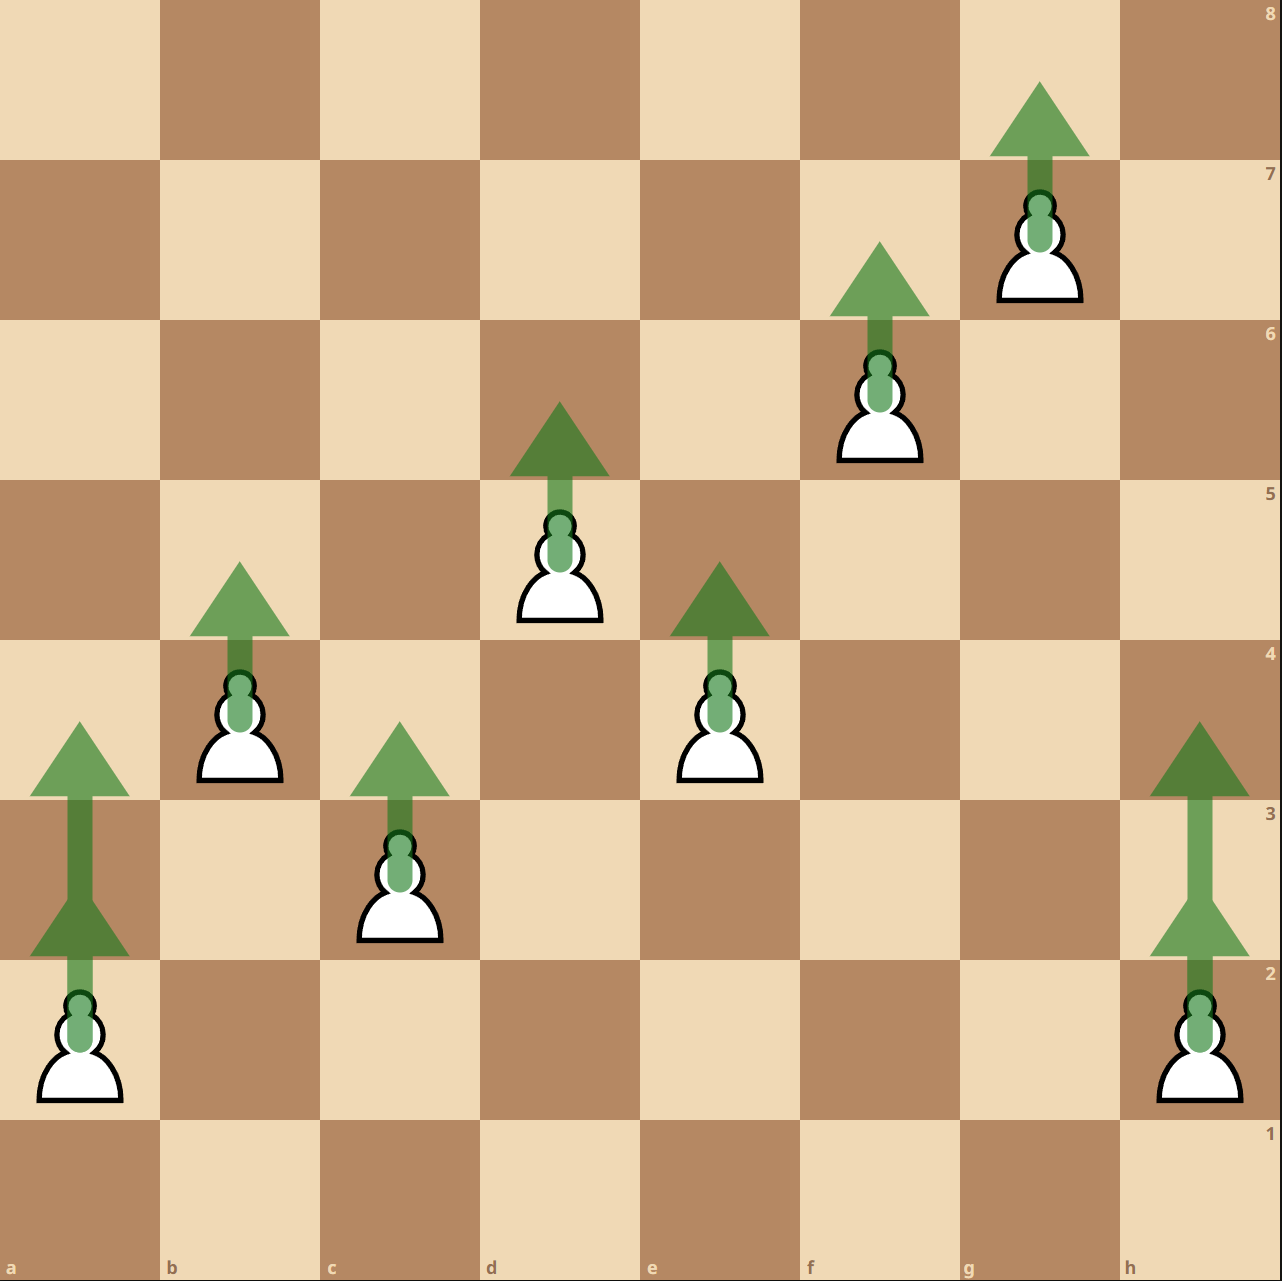
\includegraphics[width=1.07\textwidth] {movimento_pedone.png}
        \caption{aaaa}
    \end{minipage}
    \hfill
    \begin{minipage}[b]{0.21\textwidth}
        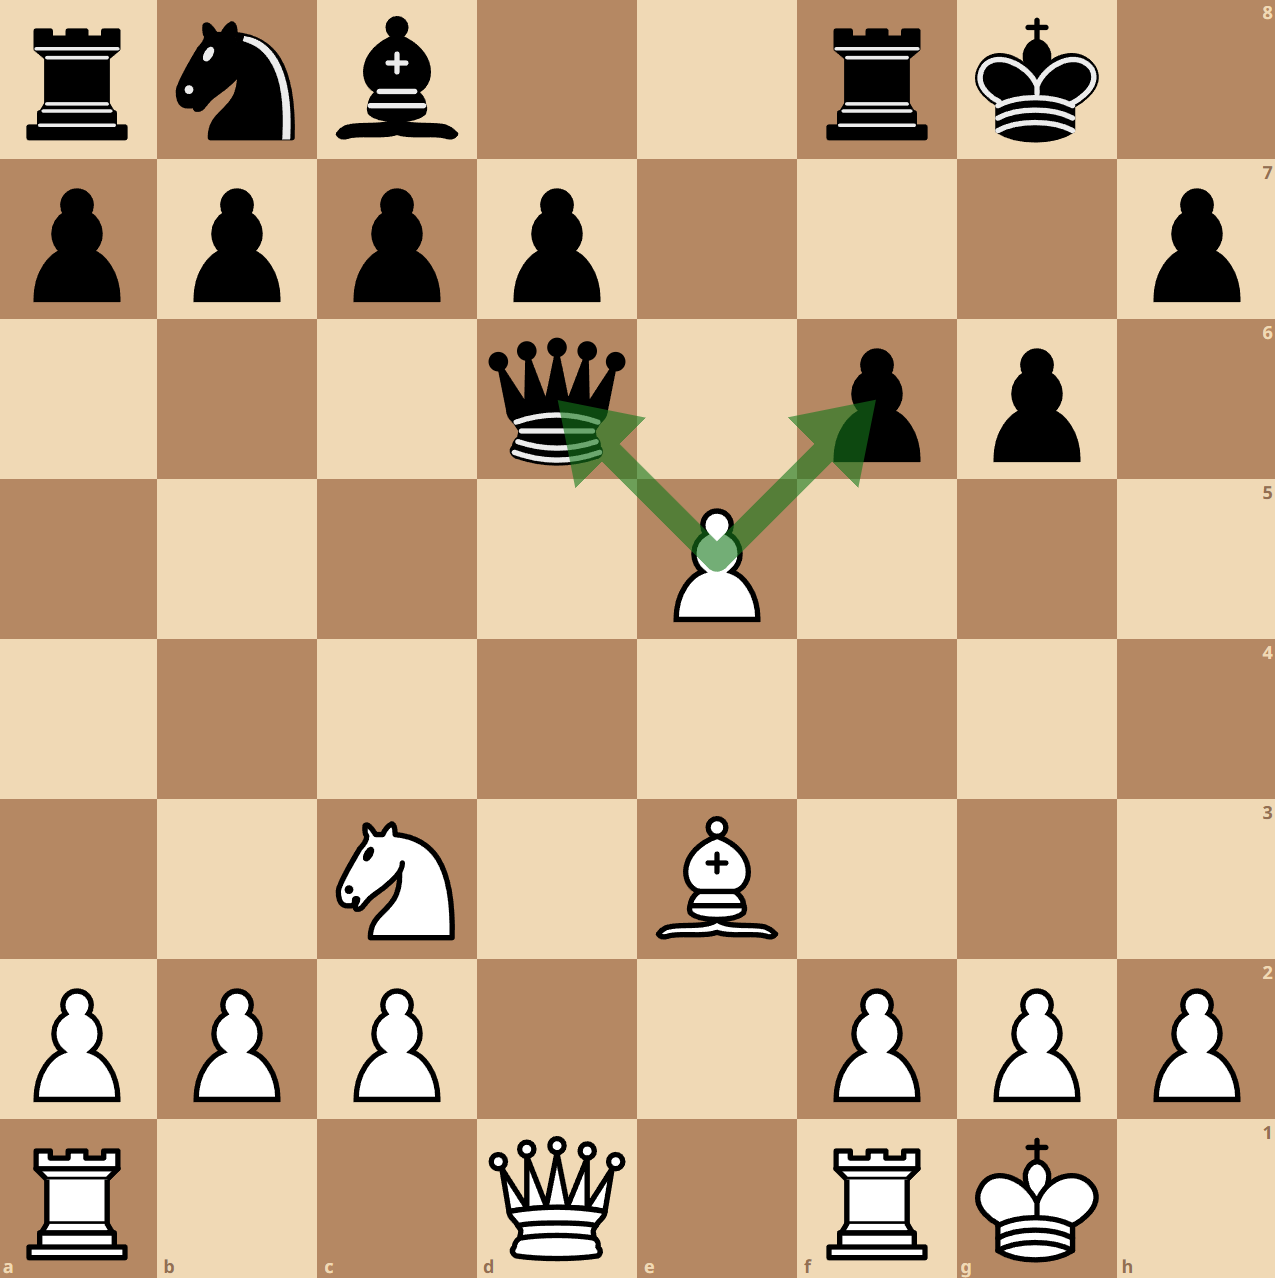
\includegraphics[width=1.07\textwidth]{pedone_cattura.png}
        \caption{aaaa}
    \end{minipage}
\end{figure}










\subsubsection{generazione delle mosse di un pedone }
Di seguito è presentato un esempio di implementazione per la generazione delle mosse dei pedoni bianchi,
per quelli neri il codice si presenta identico ma con i valori di movimento adattati di conseguenza.




\begin{figure}[H]
    \begin{minipage}[t]{.63\textwidth}
        \centering \raisebox{\dimexpr-\height+1.5ex\relax}{ 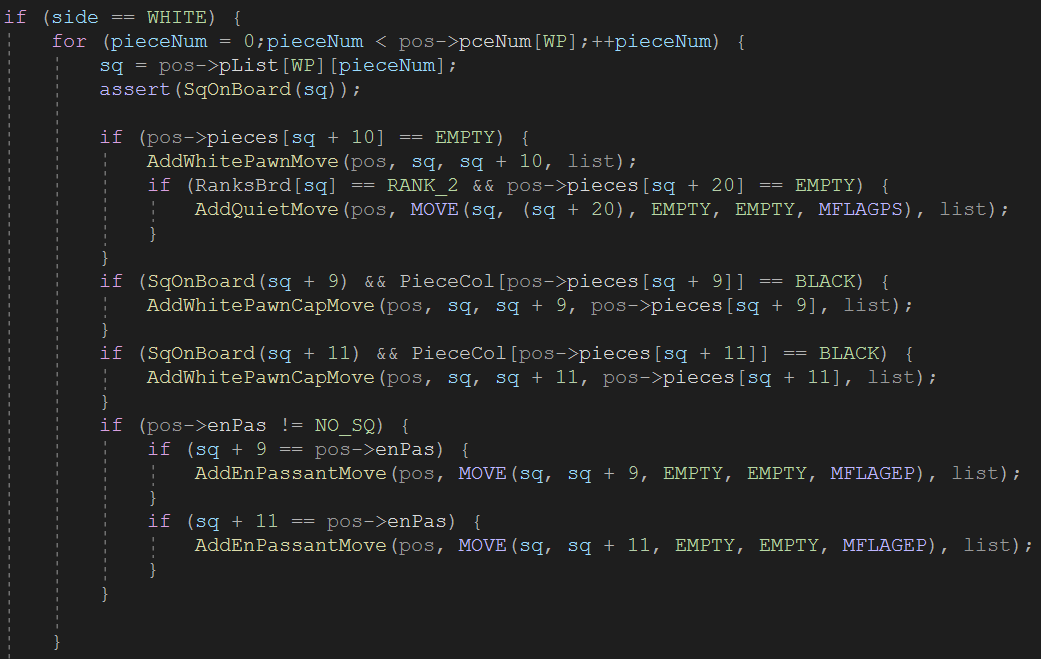
\includegraphics[width=9.5cm,height=11.5cm,keepaspectratio=false]{move_generation_pawn.png}}
    \end{minipage}
    \begin{minipage}[t]{0.35\textwidth}
        \small{
            Per generare le mosse dei pedoni,prendiamo la posizione di ogni pedone sulla scacchiera,se il pedone può avanzare in avanti di una casella allora aggiungiamo quella mossa
            all'elenco,se il pedone non era ancora stato mosso (e si trova quindi sulla traversa di partenza) e può muoversi di 2 caselle in avanti, aggiungiamo anche questa variante
            all'elenco,controlliamo poi se il pedone può catturare può catturare un pezzo diagonalmente sia destra sia a sinistra ed aggiungiamo queste eventuali mosse all'elenco,infine
            controlliamo se è possibile per il pedone effettuare una cattura en passant ed in tal caso aggiungiamo quest'ultima mossa alla lista.}
    \end{minipage}
\end{figure}






\subsection{Pezzi scorrevoli}
Si definiscono pezzi scorrevoli i pezzi che possono spostarsi di un numero non prefissato di caselle lungo l'asse orizzontale,verticale o diagonale,fino a raggiungere il bordo della scacchiera o un altro pezzo.
I pezzi scorrevoli consistono di alfiere,torre e regina,la generazione delle mosse di questo tipo di pezzi è più complessa rispetto a quella degli altri pezzi, quanto bisogna controllare la presenza di pezzi,propri
o avversari che siano, in grado di fermare il movimento del pezzo e bisogna assicurarsi che il pezzo non superi il bordo della scacchiera.


\subsubsection{alfieri}
The bishop chess piece moves in any direction diagonally. Chess rules state that there is no limit
 to the number of squares a bishop can travel on the chessboard, as long as there is not another
  piece obstructing its path. Bishops capture opposing pieces by landing on the square occupied
   by an enemy piece.
\begin{figure}[H]
    \centering
    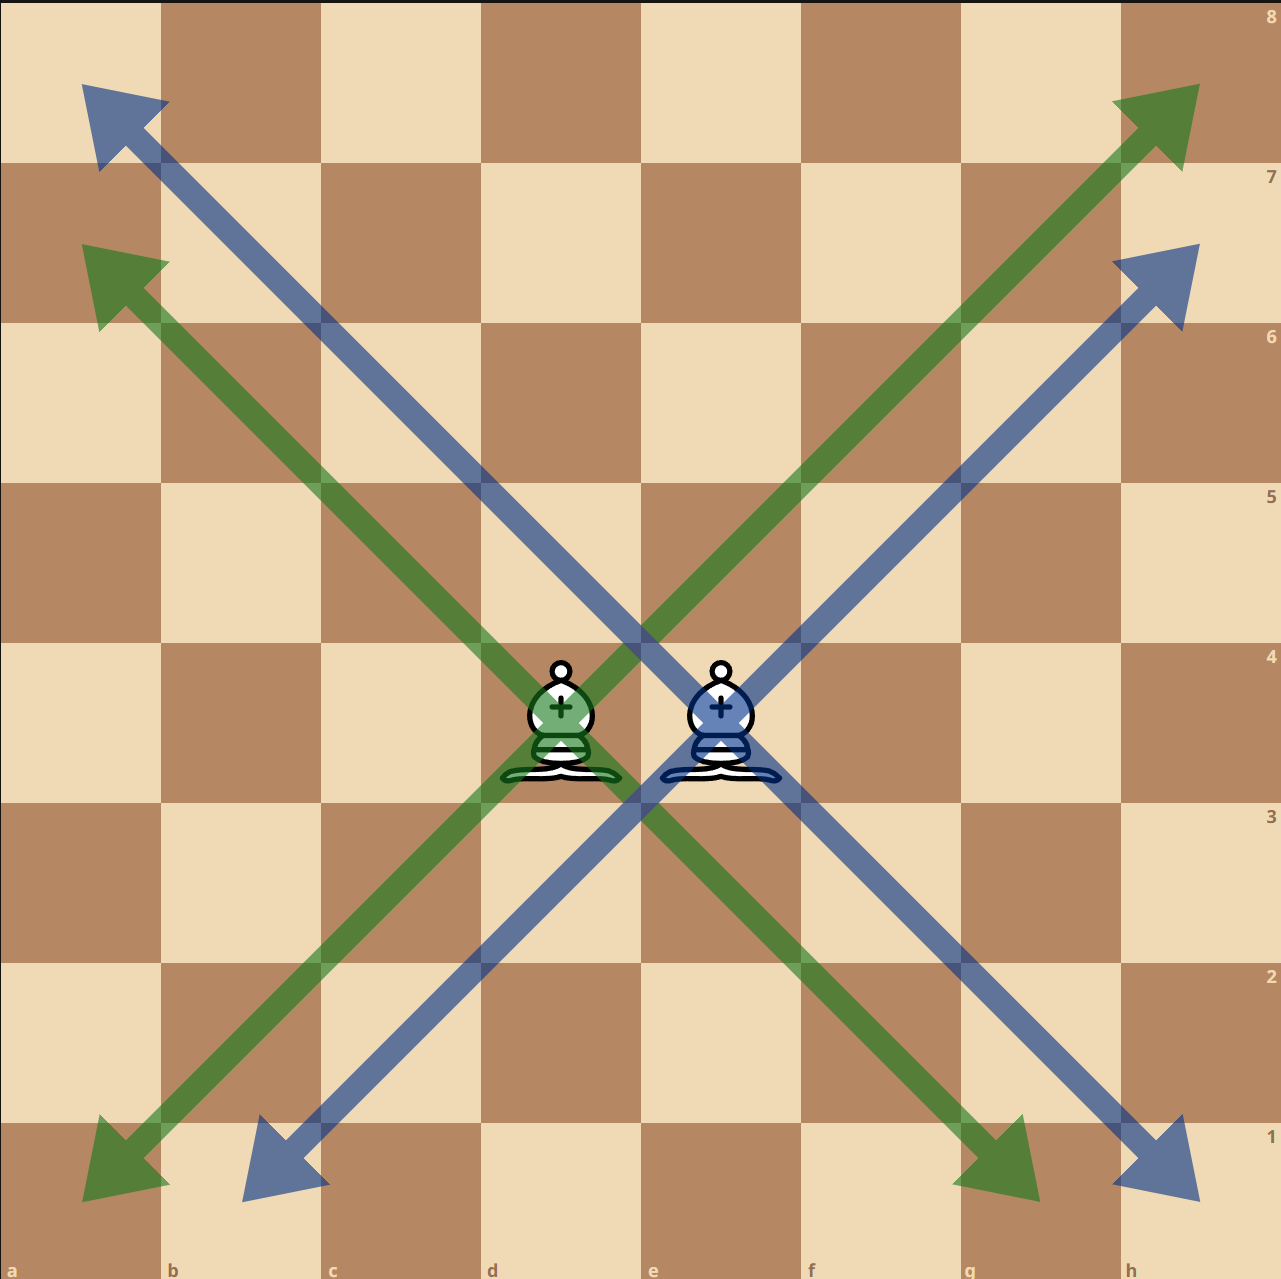
\includegraphics[width=\linewidth/2] {movimento_alfiere.png}
    \caption{move.h}
\end{figure}

\subsubsection{generazione delle mosse di un alfiere }


\subsubsection{torri}
The rook moves horizontally or vertically, through any number of unoccupied squares (see diagram).
 The rook cannot jump over pieces. As with captures by other pieces apart from en passant, 
 the rook captures by occupying the square on which the enemy piece stands.
\begin{figure}[H]
    \centering
    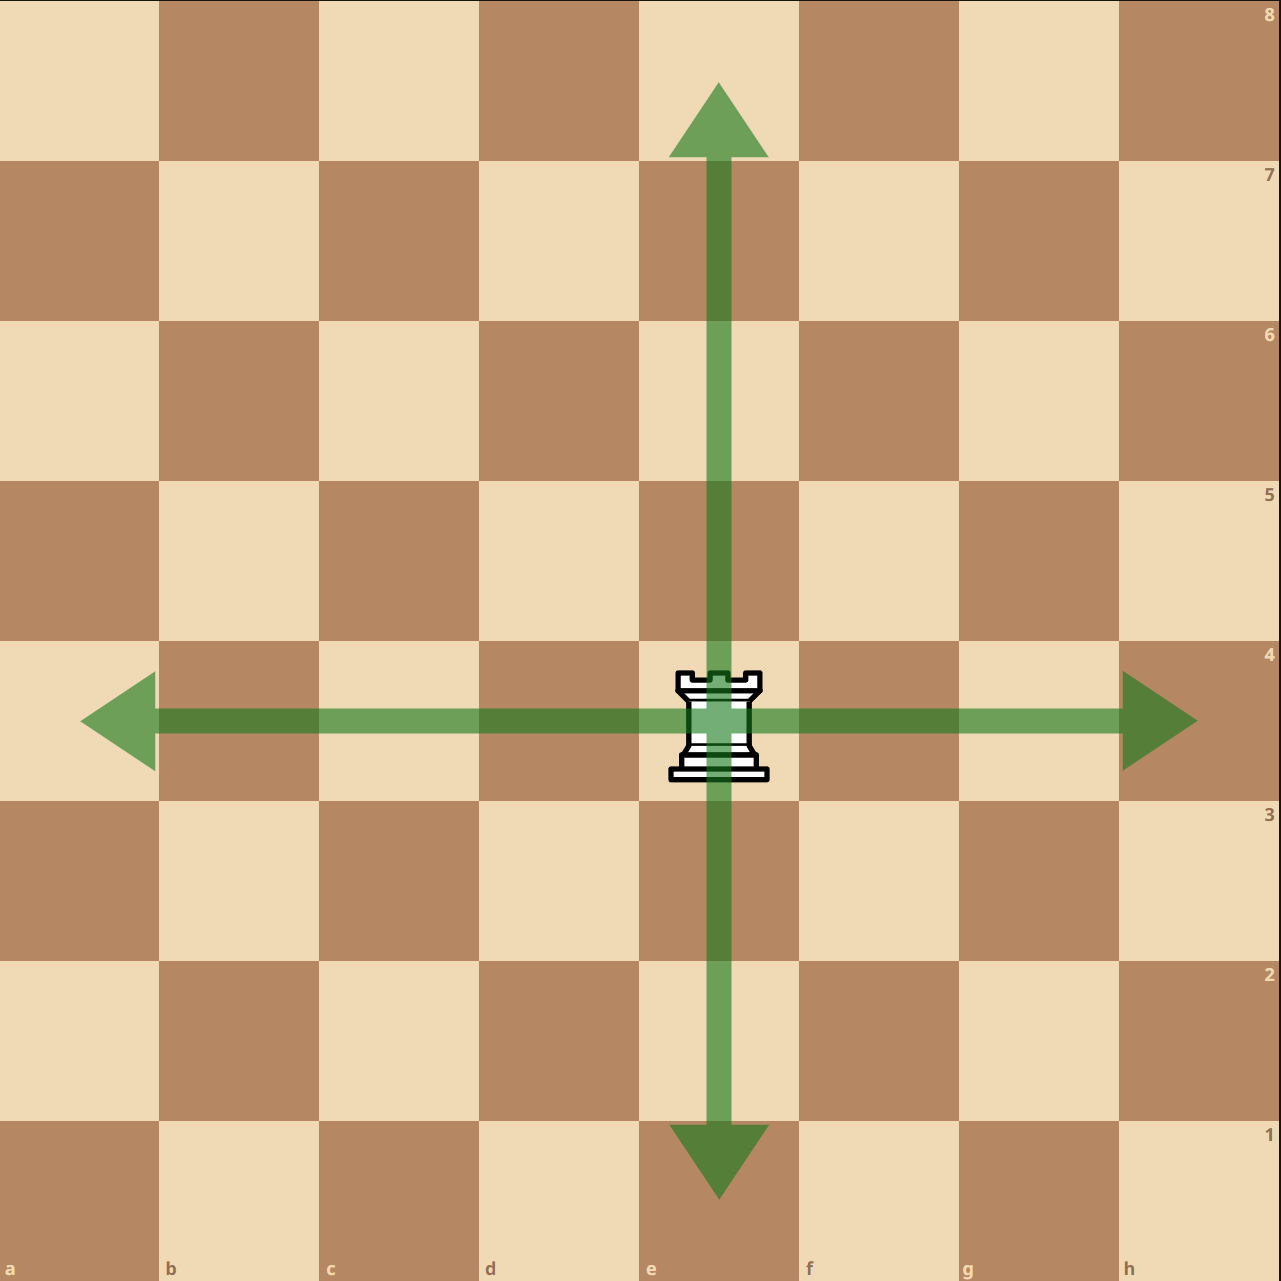
\includegraphics[width=\linewidth/2] {movimento_torre.png}
    \caption{move.h}
\end{figure}


\subsubsection{generazione delle mosse di una torre }





\subsubsection{regine}
The queen can be moved any number of unoccupied squares in a straight line vertically,
 horizontally, or diagonally, thus combining the moves of the rook and bishop. 
 The queen captures by occupying the square on which an enemy piece sits.
\begin{figure}[H]
    \centering
    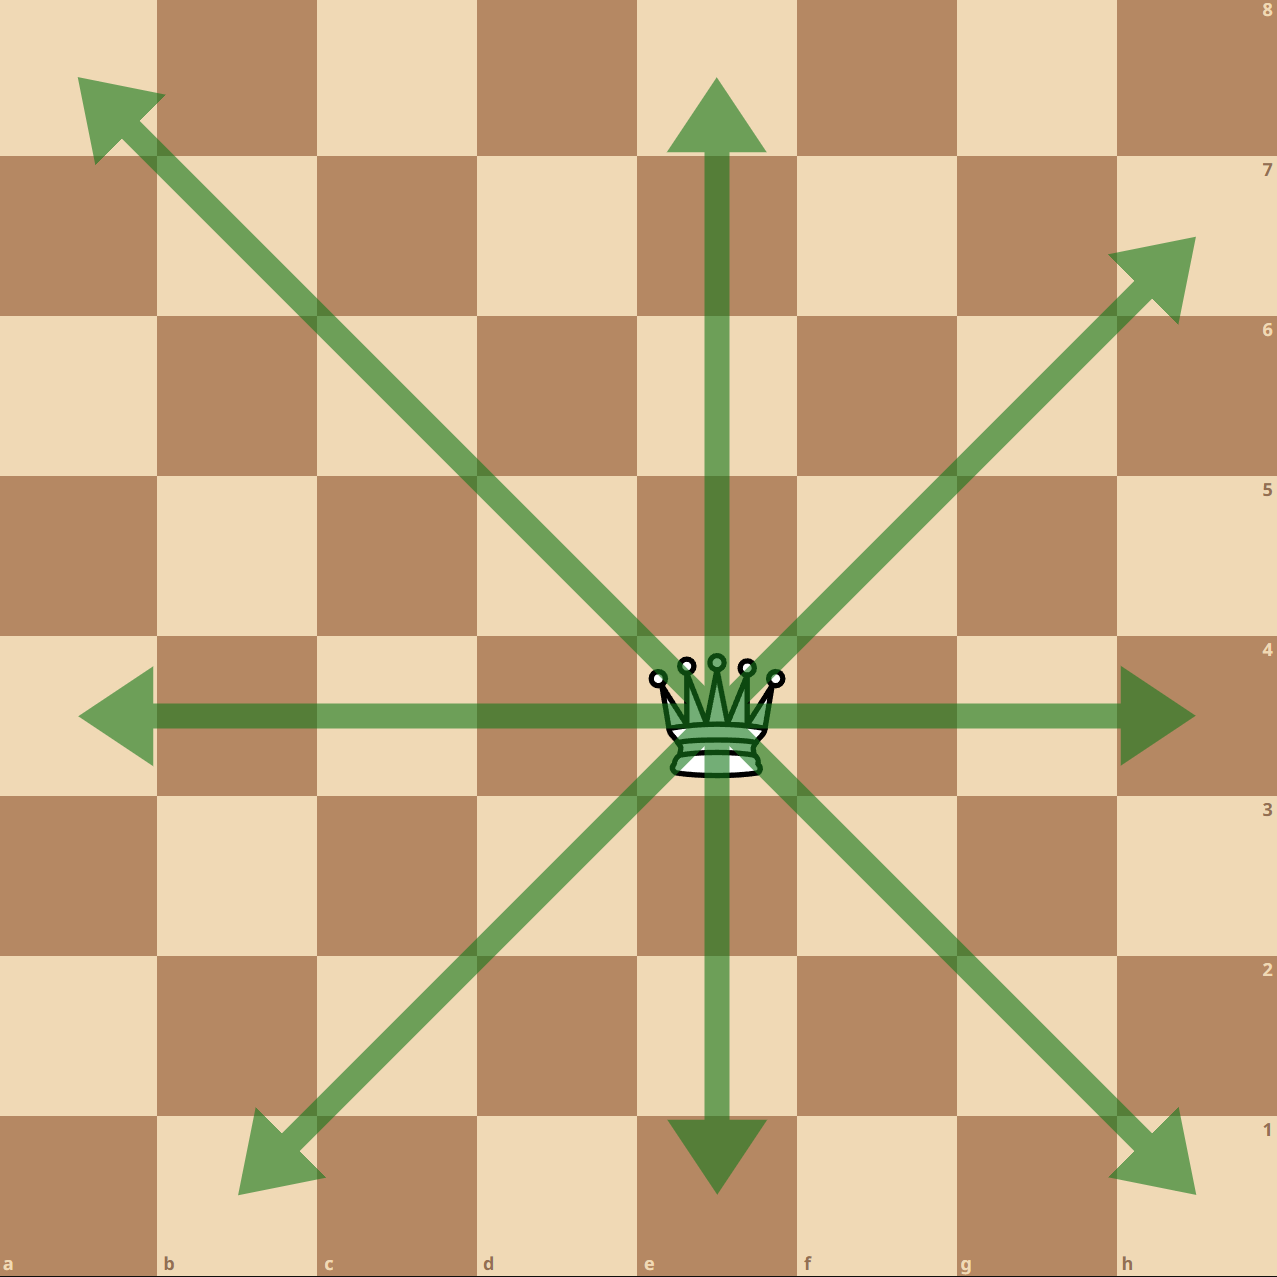
\includegraphics[width=\linewidth/2] {movimento_regina.png}
    \caption{move.h}
\end{figure}


\subsubsection{generazione delle mosse di una regina }





\subsubsection{non sliding}










\begin{figure}[h]
    \centering
    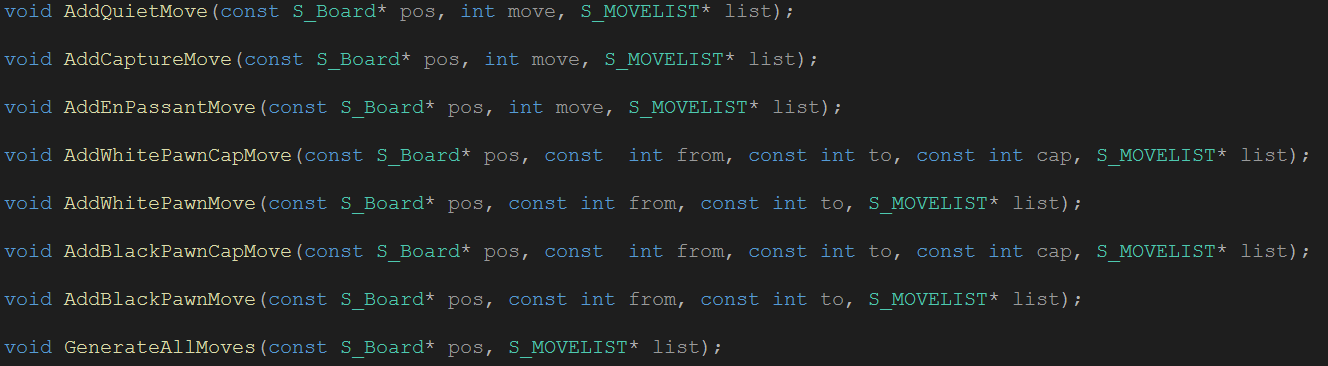
\includegraphics[width=\linewidth/2] {movegen-h.png}
    \caption{struttura movelist e bitmasks presenti in move.h }
\end{figure}


\begin{figure}[H]
    \begin{minipage}[t]{.63\textwidth}
        \centering \raisebox{\dimexpr-\height+1.5ex\relax}{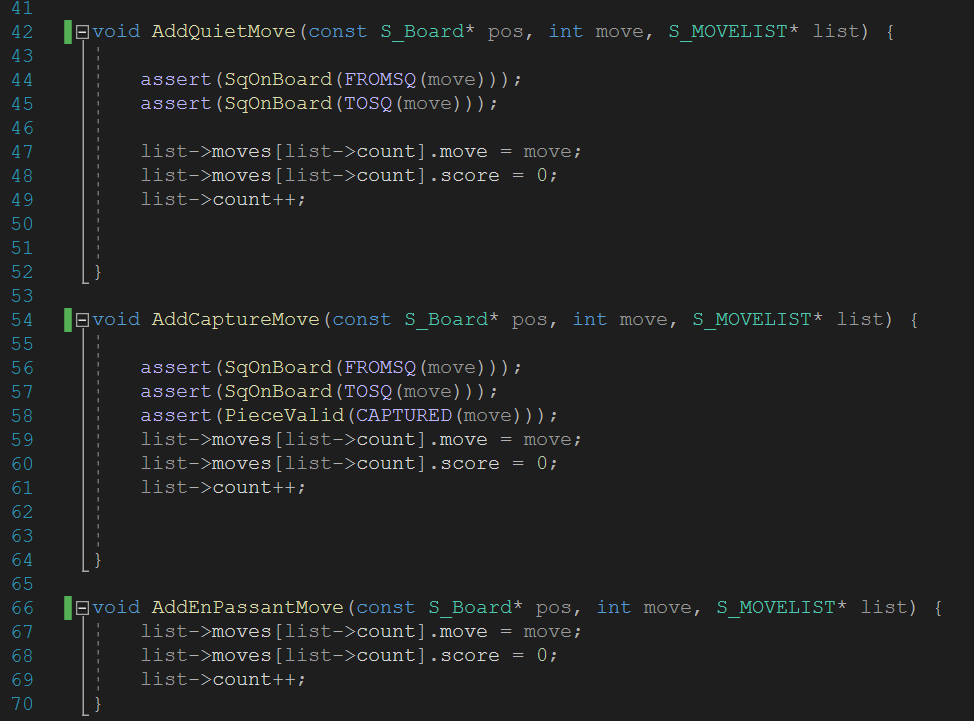
\includegraphics[scale=0.5]{PieceMoves.png}

        }
        \caption{bitboard.c}

    \end{minipage}
    \begin{minipage}[t]{0.35\textwidth}
        {
        }

    \end{minipage}
\end{figure}









\begin{figure}[H]
    \begin{minipage}[t]{.63\textwidth}
        \centering \raisebox{\dimexpr-\height+1.5ex\relax}{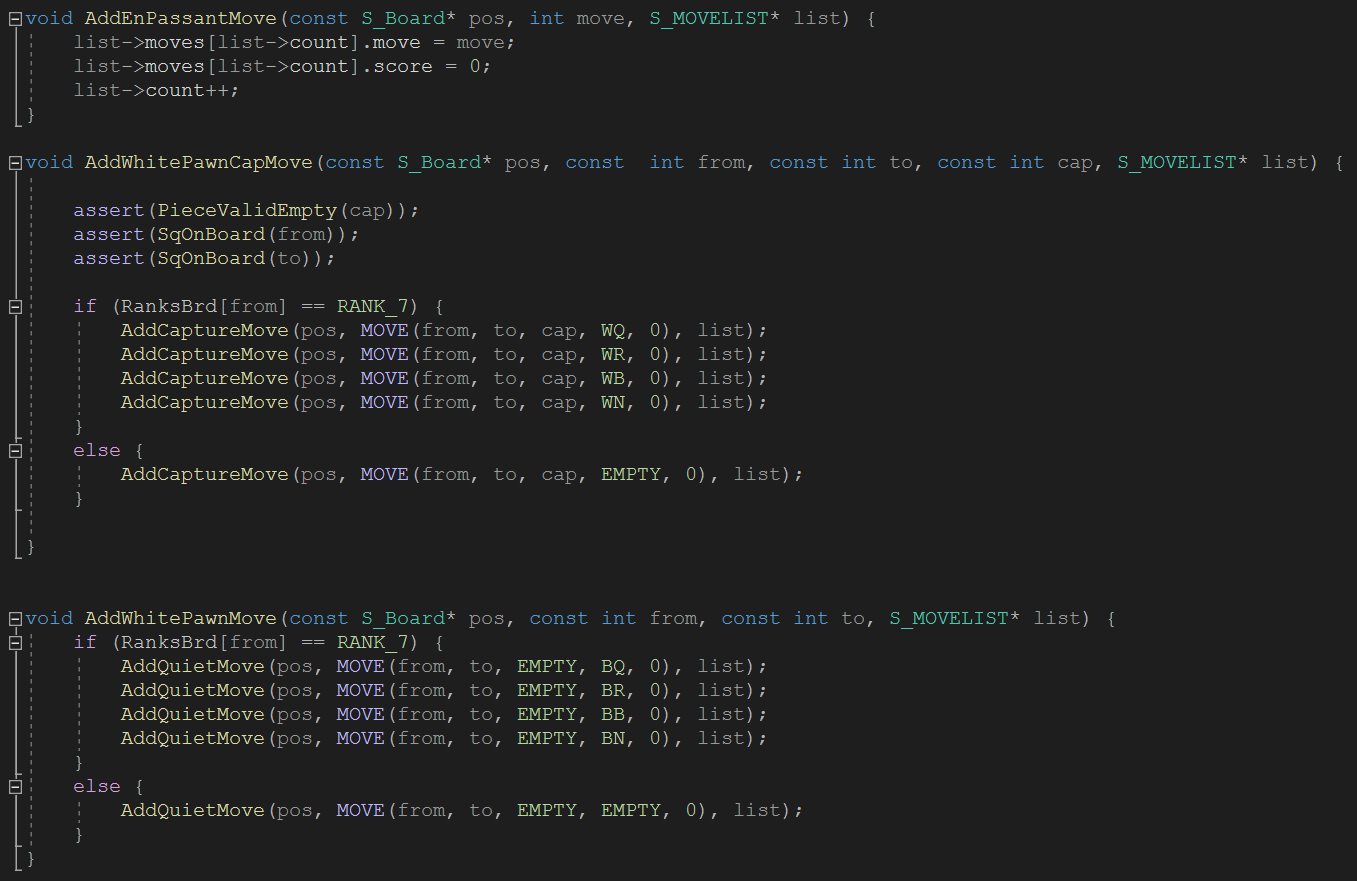
\includegraphics[scale=0.5]{PawnMoves.png}
        }
        \caption{bitboard.c}
        \label{fig:PawnMoves}
    \end{minipage}
    \begin{minipage}[t]{0.35\textwidth}
        {
        }
    \end{minipage}
\end{figure}








\section{MakeMove}








\section{Perft}
Perft è una funzione di debugging che attraversa l'albero delle mosse legali generate e conta tutti i nodi
foglia fino ad una data profondità n.Il numero viene poi comparato con dei valori noti per controllare la
presenza di bug.
I nodi vengono contati alla fine della generazione, dopo l'ultimo makemove,non vengono quindi contati
i nodi foglia che si trovano a profondità superiori di n.Perft inoltre ignora i pareggi per ripetizione,
per la regola delle 50 mosse, e per materiale insufficiente.Utilizzando la stessa versione di perft, o In
alternativa una versione estremamente simile di perft,è possibile comparare il tempo impiegato da diversi
generatori di mosse.


\begin{figure}[h]
    \centering
    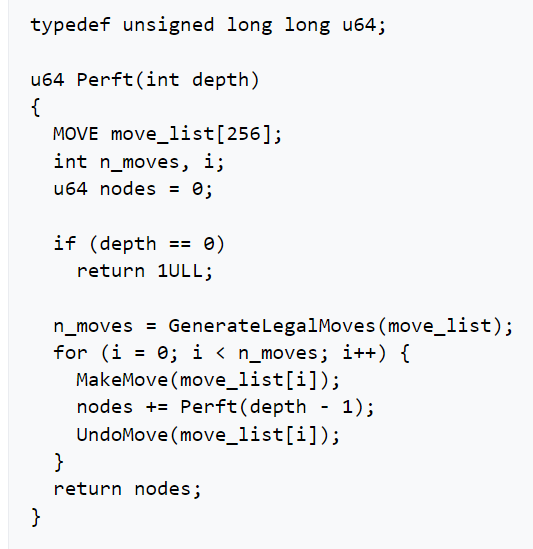
\includegraphics[width=\linewidth/2] {Perft.png}
    \caption{codice di una funzione basica di perft}
\end{figure}


